\documentclass[12pt,a4paper]{book}
%\documentclass[a4paper,french]{book}
%\usepackage[17pt]{extsizes}


\input{../1ere-preambule}

\newcommand{\va}[1]{\lvert \ #1 \ \rvert}
\newcommand{\vaf}[1]{\left\lvert \ #1\  \right\rvert}

\begin{document}
\graphicspath{{images/}}
%\setcounter{chapter}{1}
\chapter[Stats - Correction des exercices]{Statistiques \\ correction des exercices}
\thispagestyle{fancy}

\section*{Activités}
\subsection*{Activité A p 29}

\subsubsection*{Questions :}

\begin{enumMet}
	\item \begin{enumMet}
		\item L'affirmation est vraie. Le doc.1 nous informe que $27,5 \%$ des femmes ont un niveau Bac +3 ou plus.
		\item L'affirmation est fausse. Le doc.1 nous informe que $24,7\%$ des hommes ont un niveau Bac +3 ou plus, $12,8\%$ ont un niveau Bac +2 et $17,8\%$ ont un niveau Bac ou équivalent, ce qui correspond à un total de $55,3\%$ ayant au minimum un niveau Bac ou équivalent. Ce résultat est bien inférieur aux deux tiers évoqués dans l'affirmation.
		\item On ne peut a priori pas conclure car le doc.1 ne nous donne que des résultats sur les proportions et non sur les effectifs. Pour déterminer si l'affirmation est vraie ou fausse, il faudrait connaître le nombre d'hommes et de femmes dans la population pour ensuite calculer le nombre d'hommes et de femmes sans diplôme ou avec le brevet des collèges à l'aide des proportions des graphiques.
	\end{enumMet} 
	\item En 2019, il y avait environ $4$ millions de femmes et $3,5$ millions d'hommes employés de professions intermédiaires.
	\item Les inégalités salariales entre les femmes et les hommes se réduisent chez les cadres où l'écart de rémunération est toutefois le plus élevé. On retrouve également un écart qui tend à se réduire chez les employés, où l'écart de rémunération est le plus faible. En revanche, les écarts de rémunération stagnent depuis 2018 chez les professions intermédiaires et les ouvriers.
\end{enumMet}

\subsubsection*{Bilan :}

Un diagramme circulaire permet de comparer des parts de la population, sans données d'effectif. Un diagramme en bâtons est bien adapté pour lire des effectifs. Une courbe permet de mettre en évidence une évolution.

\subsection*{Activité B p 30-31}

\subsubsection*{Questions :}


\begin{enumMet}
	\item Effectivement pour la manipulation des syllabes en français, en REP+, $61$\% des élèves présentent une maîtrise suffisante, contre $86$\% des élèves dans le privé. Or $86 - 61 = 25$. Attention, on ne peut pas dire qu'entre les deux valeurs, l'augmentation est de $25$\%, ce qui correspondrait à un pourcentage d'augmentation.
	
	Le \guillemets{point de pourcentage} est donc une unité qui correspond à $1\%$ de l'effectif des élèves de CP.
	\item C'est la compétence “comprendre des mots à l'oral” pour laquelle l'écart en points de pourcentage est le plus élevé entre les deux publics : il est de 41 points de pourcentage.
	\item Regrouper les élèves en deux catégories seulement au lieu de quatre va rendre les données moins précises. Il vaut mieux détailler au maximum.
	\item Les personnes sur la tranche 25-44 ans ont tendance à s'arrêter au même niveau d'études que leur parent le plus diplômé. Plus un parent avait un diplôme élevé, plus l'enfant aura tendance à avoir un diplôme élevé également, et inversement.
	\item Le document 3 présente la répartition des élèves enfants d'ouvriers ou d'inactifs selon le secteur : public ou privé. On se rend compte que la grande majorité des enfants d'ouvriers ou d'inactifs est scolarisée dans le public et qu'ils représentent plus de la moitié des élèves en lycée professionnel. Ceci pourrait découler des difficultés scolaires rencontrées par les élèves présentes dès le CP (document 1), dues également à un manque d'informations par rapport aux études supérieures. 
	\item 
	\begin{enumMet}
		\item Les trois pays dont le score des élèves en milieu défavorisé est le plus proche de celui de la France sont la Belgique, l'Allemagne et l'Italie.
		\item Belgique : $550$ et $440$, écart : $110$; Allemagne : $564$ et $460$, écart : $104$; Italie : $511$ et $436$, écart : $75$ ; France : $550$ et $443$, écart : $107$.\\
		Les écarts entre la France, la Belgique et l'Italie sont à peu près similaires, l'écart est moindre en Italie, aussi parce que les résultats de l'épreuve Pisa sont moins élevés que pour les autres pays, y compris pour les élèves provenant d'un milieu social favorisé.
		\item Les résultats des élèves Français à l'épreuve Pisa sont parmi les moins bons pour ceux provenant de milieux défavorisés, alors que les résultats obtenus par les élèves issus de milieux favorisés sont dans la moyenne des pays de l'OCDE présentés dans le tableau. On peut souligner que les informations obtenues semblent montrer que les inégalités scolaires sont très présentes en France. 
	\end{enumMet}
\end{enumMet}

\subsubsection*{Bilan :}

Nous sommes obligés de reconnaître que de grosses inégalités sociales sont présentes dans l'enseignement secondaire et que le niveau d'études d'un élève dépend souvent du niveau d'études de ses parents et de sa classe socio-professionnelle. Il faut espérer que dans le futur, de meilleures stratégies seront mises en place afin de réduire les écarts entre les élèves.

\section*{Exercices d'automatismes}

\subsection*{Ex 4 p 35}


\begin{enumMet}
	\item Dans le collège, $190$ élèves ne mangent pas à la cantine.         
	\item Il y a $350-210 = 140$ garçons demi-pensionnaires.         
	\item Il y a $210+90=300$ filles dans l'établissement.
	\item La proportion de filles demi-pensionnaires parmi l'ensemble des élèves est $\dfrac{210}{540}         \approx 0,39$.
	\item La proportion de garçons parmi les élèves externes est $\dfrac{100}{190} \approx 0,53$.
\end{enumMet}

\subsection*{Ex 5 p 35}


\begin{enumMet}
	\item \,
	
	\begin{center}
		\begin{tabular}{ | Xc | Xc | Xc | Xc | }
			\hline
			
			
			& 
			
			Volet 1 vu & 
			
			Volet 1 non vu & 
			
			Total\\ \hline
			
			
			Volet 2 vu & 
			
			450 & 
			
			300 & 
			
			750\\ \hline
			
			
			Volet 2 pas vu & 
			
			50 & 
			
			200 & 
			
			250\\ \hline
			
			
			Total & 
			
			500 & 
			
			500 & 
			
			1000\\ \hline
		\end{tabular}
	\end{center}
	\item Il y a $450+50 = 500$ personnes qui ont vu le volet 1.
	\item Il y a également $500$ personnes qui ne l'ont pas vu. En tout, $1000$ personnes ont participé au sondage.
\end{enumMet}

\subsection*{Ex 6 p 35}


\begin{enumMet}[label=\arabic*.]
	\item Dresser le tableau croisé d'effectifs correspondant à la situation présentant les différents animaux en colonne et les adoptions ou non en ligne.
	
	\begin{center}
		\begin{tabular}{ | Xc | Xc | Xc | Xc | }
			\hline
			
			
			& 
			
			Chat & 
			
			Chien & 
			
			Total\\ \hline
			
			
			Adopté & 
			
			25 & 
			
			20 & 
			
			45\\ \hline
			
			
			Pas adopté & 
			
			25 & 
			
			40 & 
			
			65\\ \hline
			
			
			Total & 
			
			50 & 
			
			60 & 
			
			110\\ \hline
		\end{tabular}
	\end{center}
	\item Il reste $65$ animaux à adopter : $25$ chats et $40$ chiens.
\end{enumMet}

\subsection*{Ex 7 p 35}

L'échelle du diagramme en bâtons horizontal est faussée puisque le bâton représentant le nombre de tests de dépistages en France devrait être trois fois moins grand que le bâton représentant l'Allemagne. Cela donne l'impression que la France a fait plus de tests pour 1 000 habitants que dans les faits.

\subsection*{Ex 8 p 35}

On remarque que l'échelle n'est pas du tout respectée, ce qui donne l'impression visuelle que l'Argentine procède à de nombreux tests rapporté à un million d'habitants. Son bâton, qui est associé à 330 tests par million d'habitants, devrait être beaucoup plus petit que le bâton représentant la Norvège qui est à 22 300 tests par million d'habitants.

\subsection*{Ex 9 p 35}

Voici le diagramme en bâton représentant la composition globale des déchets marins :


\begin{center}
	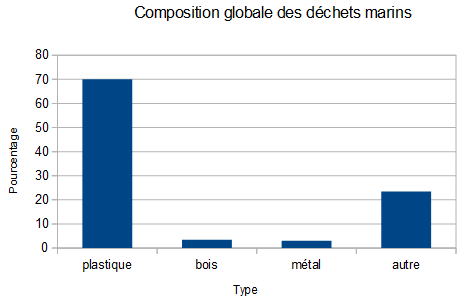
\includegraphics[scale = 0.55]{images/image14.png}
\end{center}

\subsection*{Ex 10 p 35}


\begin{center}
	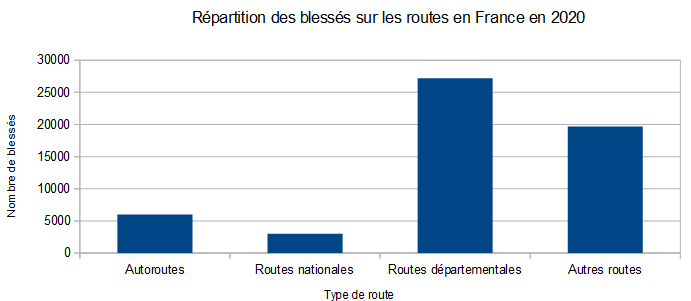
\includegraphics[scale = 0.55]{images/image18.png}
\end{center}

\subsection*{Ex 11 p 37}


\begin{enumMet}
	\item C'est l'Asie qui regroupe plus de la moitié de la population mondiale.
	\item La population est plus importante en Europe qu'en Amérique du Nord.
\end{enumMet}

\subsection*{Ex 12 p 37}


\begin{enumMet}
	\item Le secteur orange qui correspond à 48\% est visiblement faux car il prend plus de la moitié du diagramme circulaire, ce qui correspond à plus de 50\%.
	\item Voici le diagramme corrigé :
	\begin{center}
		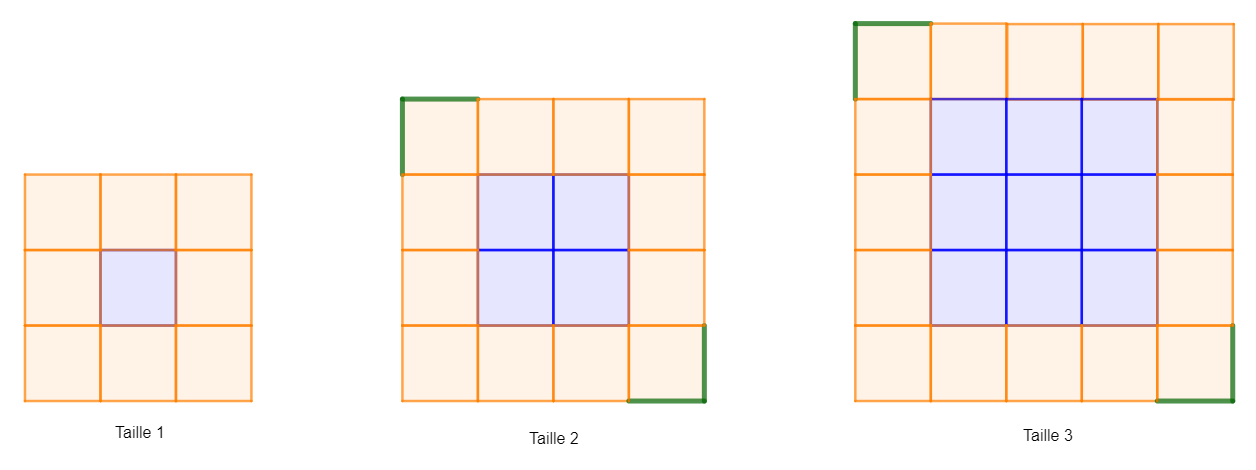
\includegraphics[scale = 1.1]{images/image1.png}
	\end{center}
	
\end{enumMet}

\subsection*{Ex 13 p 37}

	\begin{center}
		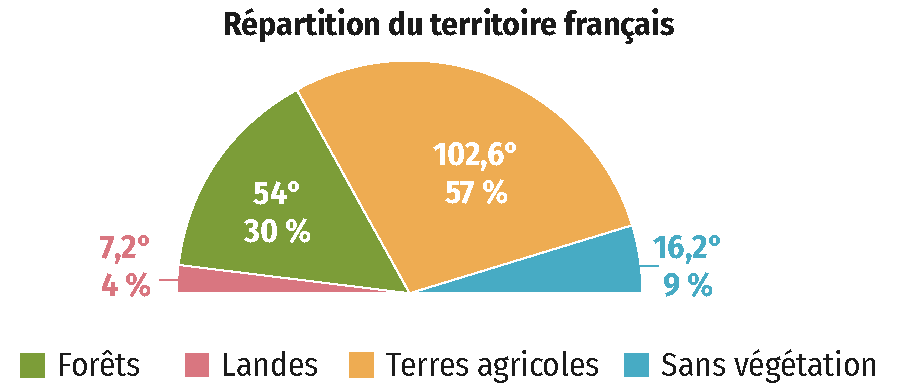
\includegraphics[scale = 1.1]{images/image9.png}
	\end{center}

\subsubsection*{Ex 15 p 37}

Pendant les trois premiers jours, la serre B était la plus humide. Les quatre jours suivants, la serre A était la plus humide.

\subsubsection*{Ex 16 p 37}

Il n'y a pas de légende sur l'axe des abscisses et pas d'unités pour la température en ordonnées.

\subsubsection*{Ex 17 p 37}

\begin{enumMet}
	\item \ 
	\begin{center}
		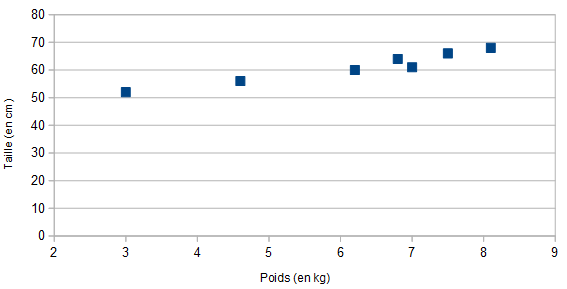
\includegraphics[scale = 0.6]{images/image21.png}
	\end{center}
	\item La taille augmente essentiellement en même temps que le poids. On peut remarquer que le nuage de points est proche d'être aligné. À partir des données obtenues et sur l'intervalle étudié, on peut donc modéliser la corrélation entre la taille en cm et le poids en kg par une fonction affine. On peut se référer pour cela aux pages Pour aller plus loin.
\end{enumMet}

\section*{Entraînement}

\subsection*{Ex 18 p 38}

\begin{enumMet}
	\item Il y a eu $379930+147596+186395 = 713921$ admis.
	\item Au total, on compte $385959+154303+205601=745863$ candidats dont 713921 admis. Le taux global de réussite au baccalauréat en France 2021 lors de la session 2021 vaut donc $\dfrac{713921}{745863} \approx 95,72 $ \%.
	\item Au baccalauréat général, on compte 385 959 candidats dont 379 930 admis. Le taux de réussite au bac général lors de la session 2021 en France métropolitaine est donc $\dfrac{379930}{385959} \approx 98,44 $ \%.
	\item On procède au calcul : $5286 \times \dfrac{98,66}{100} = 5215$ ont été admis.
	
\end{enumMet}

\subsection*{Ex 19 p 38}


\begin{enumMet}
	\item C'est l'Asie de l'Est qui a émis le plus de gaz à effet de serre (27\%) en 2019. Au contraire, l'Australie, le Japon et la Nouvelle Zélande sont les zones géographiques en ayant émis le moins (3\%).
	\item 
	\begin{enumMet}
		\item La population mondiale est de $7605$ millions d'habitants. L'Asie de l'Est représente une proportion de $\dfrac{1471}{7605} \approx 0,19$ de la population mondiale. De même, l'Asie du Sud représente une proportion de $\dfrac{1836}{7605} \approx 0,24$ de la population mondiale.
		\item On observe que le pourcentage d'émission de GES en Asie du Sud est bien moindre qu'en Asie de l'Est alors que la proportion d'habitants y est plus importante.
	\end{enumMet}
%	\newpage
	\item \,
	
	\begin{tabular}{ | p{3cm} | p{2,5cm} | p{2,5cm} | p{2,5cm} | p{2,5cm} | }
		\hline
		
		
		& 
		
		Population (en million) & 
		
		Pourcentage d'émission de gaz à effet de serre & 
		
		Quantité de gaz émis (en Gt) & 
		
		Émis par habitant (en t)\\ \hline
		
		
		Afrique & 
		
		$1292$ & 
		
		$9\%$ & 
		
		$5,31$ & 
		
		$4,11$\\ \hline
		
		
		Amérique latine et Caraïbes & 
		
		$646$ & 
		
		$10\%$ & 
		
		$5,90$ & 
		
		$9,13$\\ \hline
		
		
		Amérique du Nord & 
		
		$366$ & 
		
		$12\%$ & 
		
		$7,08$ & 
		
		$19,34$\\ \hline
		
		
		Asie de l'Est & 
		
		$1471$ & 
		
		$27\%$ & 
		
		$15,93$ & 
		
		$10,83$\\ \hline
		
		
		Asie du Sud & 
		
		$1836$ & 
		
		$8\%$ & 
		
		$4,72$ & 
		
		$2,57$\\ \hline
		
		
		Asie du Sud-Est et Pacifique & 
		
		$674$ & 
		
		$9\%$ & 
		
		$5,31$ & 
		
		$7,88$\\ \hline
		
		
		Australie, Japon, Nouvelle Zélande & 
		
		$157$ & 
		
		$3\%$ & 
		
		$1,77$ & 
		
		$11,27$\\ \hline
		
		
		Europe & 
		
		$620$ & 
		
		$8\%$ & 
		
		$4,72$ & 
		
		$7,61$\\ \hline
		
		
		Europe de l'Est, Asie Centrale et de l'Ouest & 
		
		$291$ & 
		
		$6\%$ & 
		
		$3,54$ & 
		
		$12,16$\\ \hline
		
		
		Moyen Orient & 
		
		$252$ & 
		
		$5\%$ & 
		
		$2,95$ & 
		
		$11,71$\\ \hline
		
		
		Commerce international et aviation & 
		
		- & 
		
		$3\%$ & 
		
		$1,77$ & 
		
		\\ \hline
	\end{tabular}
	
	
	\item La zone émettant le plus de gaz par habitant est l'Amérique du Nord. C'est l'Asie du Sud qui en émet le moins.
	
	
\end{enumMet}

\subsection*{Ex 20 p 38}


\begin{enumMet}
	\item 
	\begin{enumMet}
		\item L'espérance de vie à la naissance est l'espérance de vie d'un individu entre le moment de sa naissance et de sa mort. L'espérance de vie en bonne santé est l'espérance de vie d'un individu entre le moment de sa naissance et celui où il ne sera plus considéré en bonne santé (incapacité dans les gestes de la vie quotidienne).
		\item L'espérance de vie à la naissance est supérieure à l'espérance de vie en bonne santé car actuellement, beaucoup de personnes vivent longtemps en mauvaise santé.
	\end{enumMet}
	\item Il y a 6 ans d'écart entre les espérances de vie à la naissance des femmes et des         hommes en 2020. Cela peut s'expliquer par le fait que les hommes exercent des métiers plus pénibles physiquement ou à risque ; ils fument davantage et sont davantage sujets au diabète, par exemple, donc globalement ils décèdent plus jeunes. Il est possible que cet écart s'amenuise au cours des années futures car ces habitudes sont en cours de changement.
%	\newpage
	\item Quand on compare les espérances de vie en bonne santé entre les hommes et les femmes, cet écart tombe à $1,5$ ans en 2020. Cela veut s'expliquer notamment par le fait que les hommes et les femmes ont accès au même système de santé.
	\item 
	\begin{enumMet}
		\item Évolution de l'espérance de vie à la naissance des femmes entre 2010 et 2020 :\\
		$\dfrac{85,1-84,6}{84,6} \approx 0,59$ \%.
		
		Évolution de l'espérance de vie à la naissance des hommes entre 2010 et 2020 :
		
		$\dfrac{79,1-78}{78} \approx 1,41$ \%.
		\item Évolution de l'espérance de vie en bonne santé des femmes entre 2010 et 2020 : 
		
		$\dfrac{65,9-63,3}{63,3} \approx 4,11$ \%.
		
		Évolution de l'espérance de vie en bonne santé des hommes entre 2010 et 2020 : 
		
		$\dfrac{64,4-61,8}{61,8} \approx 4,21$ \%.
		\item Les progrès de la médecine font qu'il sera plus facile de garder des adultes valides plus longtemps, d'où les taux d'évolution plus élevés pour les espérances de vie en bonne santé. Par contre, il ne sera pas possible de rallonger indéfiniment notre espérance de vie, qui va progresser plus doucement avant de se stabiliser, d'où les taux d'évolution moins élevés des espérances de vie à la naissance.
	\end{enumMet}
\end{enumMet}

\subsection*{Ex 23 p 39}

\begin{enumMet}
	\item $150$ étudiants ont pratiqué le football et la natation.
	\item $300$ étudiants ont pratiqué le badminton.
	\item En sommant tous les nombres du tableau, on calcule que $1005$ étudiants ont choisi l'option sport.
\end{enumMet}

\subsection*{Ex 26 p 40}

\begin{center}
	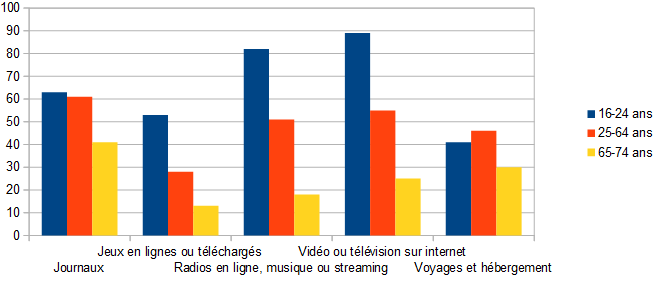
\includegraphics[scale = 0.6]{images/image23.png}
\end{center}

\section*{Pour aller plus loin : Ajustement affine avec la méthode de Meyer}

\subsection*{Ex 34 p 42}

La moyenne est $\dfrac{1+2+5+9+7+5+10+12+8+2+8}{11}\approx 6,27$.

\subsection*{Ex 35 p 42}

La moyenne est $\dfrac{-2 \times 2 + 3 \times 1 + 7 \times 5 + 8 \times 3 + 10 \times 7}{2+1+5+3+7} \approx 7,11$.

\subsection*{Ex 36 p 42}

La moyenne de Clément est de $\dfrac{12 \times 1 + 10 \times 2 + 13 \times 2 + 13 \times 3}{1+2+2+3} =12,125$.

\subsection*{Ex 37 p 42}

La moyenne des abscisses est $\dfrac{-4-1+0+5+8+9}{6} \approx 2,83$.

Celle des ordonnées est $\dfrac{3+1+6+2+5+4}{6} = 3,5$. Les coordonnées du point moyen $G$ sont donc approximativement $G(2,83;3,5)$.

\subsection*{Ex 38 p 42}


\begin{enumMet}
	\item On commence par calculer le coefficient directeur de $d$. $A$ et $B$ sont deux points du plan appartenant à $d$ donc $m=\dfrac{y_B-y_A}{x_B-x_A} = \dfrac{9-(-3)}{0-8} = \dfrac{12}{-8} = -\dfrac{2}{3}$. 
	
	Donc $d:y=-\dfrac{2}{3}x+p$. Or $B(9;0)\in d$ donc $0 = -\dfrac{2}{3}\times 9+p$ d'où $p=6$.
	
	L'équation réduite de $d$ est donc $y = -\dfrac{2}{3}x +6$.
	\item $-\dfrac{2}{3} \times 3 +6 = 4$, donc $C$ appartient bien à la droite $d$.
	\item $-\dfrac{2}{3} \times 0 +6 = 6$, donc $E$ a pour ordonnée $6$.
\end{enumMet}

\subsection*{Ex 39 p 43}


\begin{enumMet}
	\item L'ordonnée du point de la droite d'abscisse $-4$ est $-1$.
	\item L'abscisse du point de la droite d'ordonnée $5$ est $4$.
	\item On peut utiliser les deux points précédents pour déterminer l'équation réduite de $d$. On pose $A(-4;-1)$ et $B(4;5)$. Ces deux points appartiennent à $d$ donc le coefficient directeur de $d$ est donné par $\dfrac{5-(-1)}{4-(-4)} =\dfrac{6}{8}= \dfrac{3}{4}$.
	
	Pour déterminer l'ordonnée à l'origine $p$, on observe que $A$ appartient à la droit donc $-1=-4\times\dfrac{3}{4}+p$ donc $p=2$.
	
	Ainsi, l'équation réduite de $d$ est $y = \dfrac{3}{4}x +2$.
\end{enumMet}

\subsection*{Ex 40 p 43}


\begin{enumMet}
	\item Voir la figure ci-dessous.
	\item On sépare la série en deux séries de trois points : le point moyen du premier groupe est $G_1(\dfrac{5}{3};\dfrac{-1}{3})$et celui du deuxième groupe est $G_2(8;\dfrac{16}{3})$.
	\item \,
	
	\begin{center}
		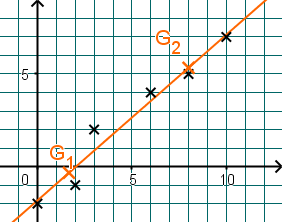
\includegraphics[scale = 0.65]{images/image8.png}
	\end{center}
	
\end{enumMet}

\subsection*{Ex 41 p 43}


\begin{enumMet}
	\item Voir la figure ci-dessous.
	\item On sépare la série en deux séries : le point moyen du premier groupe est $G_1(\dfrac{-7}{3};8,5)$ et celui du deuxième groupe est $G_2(5,75;1,75)$.
	\item \,
	
	\begin{center}
		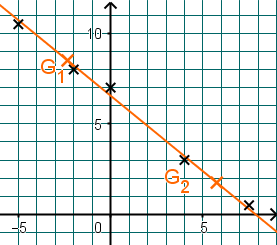
\includegraphics[scale = 0.65]{images/image24.png}
	\end{center}
	
\end{enumMet}

\newpage
\subsection*{Ex 42 p 43}


\begin{enumMet}
	\item Voir la figure ci-dessous.
	\item Les coordonnées des points moyens sont $G_1(2;805)$ et $G_2(5;913)$.
	\begin{center}
		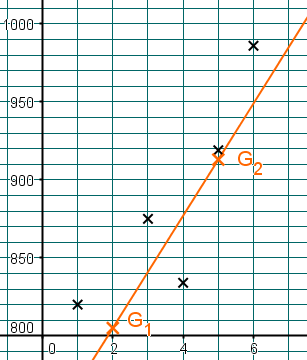
\includegraphics[scale = 0.65]{images/image12.png}
	\end{center}
	
	\item On peut estimer le nombre d'entrées à $985$ le septième jour.
	
	
\end{enumMet}

\subsection*{Ex 43 p 43}


\begin{enumMet}
	\item Les coordonnées des points moyens sont $G_1(2012;\dfrac{37}{3})$ et $G_2(2018;16)$.
	\begin{center}
		
\includegraphics[scale = 0.5]{images/image5.png}
	\end{center}
	
	\item Le chiffre d'affaires pour 2025 est estimé à $20 \ 500$ euros.
	\item Avec ce modèle, on estime que le chiffre d'affaires dépassera les $25 \ 000$ euros en 2033.
	\item On calcule les coefficients de l'équation réduite de la droite de Mayer. On utilise évidemment les coordonnées des deux points moyens $G_1$ et $G_2$ qui appartiennent à cette droite.
	
	On obtient : $m=\dfrac{16-\dfrac{37}{3}}{2018-2012} = \dfrac{\dfrac{11}{3}}{6} = \dfrac{11}{18}$ et $p=16 - 2018 \times \dfrac{11}{18} = - \dfrac{10955}{9}$, 
	
	donc l'équation est $y = \dfrac{11}{18} x -\dfrac{10955}{9}$.
	\item On utilise l'équation réduite de la droite de Mayer obtenue : $y = \dfrac{11}{18} \times 2025 -\dfrac{10955}{9} \approx 20,28$ milliers d'euros en 2025.
	
	On résout l'inéquation $ \dfrac{11}{18} x -\dfrac{10955}{9} > 25$, donc $ \dfrac{11}{18} x > \dfrac{11180}{9}$, donc $x > 2032,72$. C'est bien à partir de 2033 que le chiffre d'affaires dépassera les $25$ milliers d'euros.
	
	
\end{enumMet}

\subsection*{Ex 44 p 43}


\begin{enumMet}
	\item 
	\begin{enumMet}
		\item Les coordonnées des points moyens sont $G_1(2,5;1,43925)$ et $G_2(6,5;1,63775)$. On calcule les coefficients de l'équation réduite de la droite de Mayer à l'aide des coordonnées de ces deux points : 
		
		$m=\dfrac{1,63775-1,43925}{6,5-2,5} = \dfrac{0,1985}{4} = 0,049625$ et $p=1,63775-6,5 \times 0,049625 = 1,3151875$. Donc la droite de Mayer associée a pour équation $y = 0,049625 x +1,3151875$.
		\item En mars 2022, $x=11$ donc $y = 0,049625 \times 11 +1,3151875 = 1,8610625 \approx 1,861$. 
		
		En juin 2022, $x=14$, donc $y = 0,049625 \times 14 +1,3151875 = 2,0099375 \approx 2,010$.
	\end{enumMet}
	\item Mars 2022 : $t =\dfrac{1,913-1,861}{1,861} \approx 0,0279 = 2,79 \%$.
	
	Juin 2022 : $t =\dfrac{2,133-2,010}{2,010} \approx 0,0612 = 6,12 \%$.
	
	
\end{enumMet}

\subsection*{Ex 45 p 43}


\begin{enumMet}
	\item On note $y$ le chiffre d'affaires de 2022. Alors les coordonnées des points moyens sont $G_1(2014;\dfrac{20}{3})$ et $G_2(2020;5+\dfrac{y}{3})$. On calcule la pente de la droite de Mayer : $m=\dfrac{5+\dfrac{y}{3} -  \dfrac{20}{3}}{2020-2014} = \dfrac{\dfrac{y-5}{3}}{6} = \dfrac{y-5}{18}$.
	
	Pour que cette pente soit strictement positive, il faut donc que $y>5$.
	\item De la même façon pour que la pente soit strictement négative, il faut que $y<5$.
	
	
\end{enumMet}


\end{document}

